\part{Developing a solution to use native Cloud Applications at the Edge}
\label{part:cheops}

\epigraph{For within each seed, there is a promise of a flower.}{\emph{Dillon, Alien$^3$}}



In this part, we are going to see how we designed a solution that
fulfill the requirements defined in~\autoref{sec:principles}.

%
In~\autoref{chap:overview}, I present the overview of the approach,
and the concepts to give some insights on to reproduce an
implementation.
%
This includes the basics on how the approach function, on what it
relies from Cloud applications and what is required achieve the
requirements we explained earlier.
%
Specifically, I will detail the Domain Specific Language
(\acrshort{DSL}) made to allow for outside management of
geo-distribution concerns, and an overview of some collaborations it
offers and an insight in other possible useful collaborations is also
presented.
%
Furthermore, a glimpse into the classification of resources
dependencies is given to understand how we can help users with the
manipulation of resources.

Then, in~\autoref{chap:cheops}, I will expose the vision and current
implementation, called Cheops, a service mesh to geo-distribute Cloud
applications at the Edge.
%
% In the process, I will also give information on how this prototype
% came to be, including a first version which used an existing service
% mesh.
%
Finally, I will examine the validation we made on our implementation,
that is a common work between Geo Johns Antony, a PhD student
colleague, and me.

This part includes work from different communications made in the
scientific community~\cite{CLRB19, CDLR+20, CDL21, DCL21,
  compas-poster, DAL22} and the OpenInfra Summit
2022~\cite{OIS-Berlin22}, along with different people in the team,
namely Geo Johns Antony, Ronan-Alexandre Cherrueau, Adrien Lebre, and
Javier Rojas Balderrama, without forgetting the implication of
Matthieu Simonin.


\chapter{An approach dedicated to geo-distribution}
\label{chap:overview}


This chapter exposes the logic of the approach, how it works, what is
needed to achieve it.
%
First, I will explain how the modularity of applications is one of the
main characteristics of this approach by allowing the externalization
needed.
%
Then, I will present \scl, the Domain Specific Language made to extend
requests with the geo-distribution information.
%
Finally, I will explicit what types of collaboration we have
envisioned for the solution.

It is worth mentioning that most of this chapter comes from our
Euro-Par article~\cite{CDL21}.
% , written with Ronan-Alexandre Cherrueau
% and Adrien Lebre.

% definition
% services based
% REST API

\section{A service-mesh approach}
\label{sec:service-mesh}

% One of the available solution to deal with service composition
% dynamically is to use a reverse proxy.
% %
% A reverse proxy is a broker between clients and services of the
% application that changes the service composition on the fly.
% %
% It is implemented usually for reliability and performance, by, for
% example, balancing incoming requests to multiple instances of the same
% service within one application instance.
% %

As we discussed in~\autoref{sec:cloud-app}
and~\autoref{chap:cloud-app-to-edge}, service-based applications, like
a lot of Cloud applications, are composed of different services.
%
These services aim to provide modularity to the applications, and the
decoupling of functionalities.
%
This modularity principle comes from software engineering, allowing
separation of concerns (for example to have different teams working on
separate aspects in the business code), reusing of existing modules,
and overall better development manageability.
%


The services communicate between each other through the \acrshort{API}
they expose that allows access specific function to manipulate the
resources they handle.
%
In particular, a lot of these services use RESTful APIs to make
requests to each other, which a resource-oriented
paradigm~\cite{RCDK08, AW10, HFKLV14}.

These are the kind of applications that allow our approach:
(micro)service-based Cloud applications with RESTful APIs.
%
These applications expose endpoints to follow the REST architectural
styles, allowing users and other services to interact with the
services functionalities.
%
The series of calls in an application that execute a particular
request is called a workflow.

% The entire collection of workflows execute all the intents and
% functionnalities of an application.
%
We discussed previously how the premise of a solution is to deploy an
entire application, which automatically checks the local-first
principle.
%
Deploying all services of one application constitutes an
\emph{application instance}, which we will often use as simply
\emph{instance} afterwards.
%
The services running in an application instance are called \emph{service
instances}
%
Each application instance achieves the application intent by exposing
all of its workflows to enable the manipulation of resource values.

\vspace{5pt}

\begin{figure}[htbp]
  \centering
  %% ~~~~~~~~~~~~~~
  %% App definition
  \begin{subfigure}[b]{.7\textwidth}
    \centering
    \scalebox{1.2}{%
    \begin{tikzpicture}
      \node[labeled] (App) {$App$};
      \service[right=of App.north, matrix anchor=north west]{s}{e,f}
      \service[right=of s]{t}{g,h}
      \begin{pgfonlayer}{background}
        \fill[app, fill=CbTeal, fill opacity=0.3]
        ([xshift=-1mm,yshift=1mm]App.north west)
        rectangle ([xshift=1mm, yshift=-1mm]t.south east);
      \end{pgfonlayer}
      % Workflow
      \draw [->] (s-2-1) -- (t-3-1);
    \end{tikzpicture}
    }
    \caption{Application $App$ made of two services $s$ and $t$ and
      four endpoints $e, f, g, h$. The $s.e \rightarrow t.h$
      represents an example of a workflow.}
    \label{fig:application}
  \end{subfigure}%\hfill%
  %% ~~~~~~~~~~~~~~~~~
  %% App instantiating
  \vspace{12pt}
  \begin{subfigure}[b]{.7\textwidth}
    \centering
    \scalebox{1.2}{
    \begin{tikzpicture}
      % Instance A1
      \node[labeled] (App_1) {$App_1$};
      \service[right=of App_1.north, matrix anchor=north west]{s_1}{e,f}
      \service[right=of s_1]{t_1}{g,h}
      \begin{pgfonlayer}{background}
        \fill[app, fill=CbTeal, fill opacity=0.3]
        ([xshift=-1mm,yshift=1mm]App_1.north west)
        rectangle ([xshift=1mm, yshift=-1mm]t_1.south east);
      \end{pgfonlayer}

      % Instance A2
      \node[labeled, right=10mm of t_1.north east, anchor=north west] (App_2) {$App_2$};
      \service[right=of App_2.north, matrix anchor=north west]{s_2}{e,f}
      \service[right=of s_2]{t_2}{g,h}
      \begin{pgfonlayer}{background}
        \fill[app, fill=CbOrange, fill opacity=0.3]
        ([xshift=-1mm,yshift=1mm]App_2.north west)
        rectangle ([xshift=1mm, yshift=-1mm]t_2.south east);
      \end{pgfonlayer}

      % Workflow
      \node (c) [left=12mm of s_2-2-1] {$\bullet$};
      \draw [->] (c.east)      edge (s_2-2-1.west)
                 (s_2-2-1.east) -- (t_2-3-1.west);
    \end{tikzpicture}
    }
    \caption{Two independent instances $App_1$ and $App_2$ of the
      $App$ application. The $\bullet$ represents a client that
      executes the $s.e \rightarrow t.h$ workflow in $App_2$.}
    \label{fig:instances}
  \end{subfigure}
  \caption{Microservices architecture of a Cloud application}
  \label{fig:soa}
\end{figure}

\autoref{fig:soa} illustrates workflows in service-based applications.
%
%
On the top, \autoref{fig:application} represents a typical application
$App$ made of two services $s$, $t$ exposing endpoints $e$, $f$, $g$,
$h$.
%
It shows an example of a really simple workflow $s.e \rightarrow t.h$,
where a function in service $s$ calls an endpoint $h$ on service
$h$.
%
This is a figure similar to the~\autoref{fig:typical-app}
(page~\pageref{fig:typical-app}), but also exposing the endpoints.
%
% $App$ could be for example the OpenStack application.
% %
% In this context, service $s$ is the compute service that manages VMs.
% %
% Its endpoint $e$ creates VMs and $f$ lists them.
% %
% Service $t$ is the image service that controls operating system
% BLOBs.
% %
% Its endpoint $g$ stores an image and $h$ downloads one.
% %
% The composition $s.e \rightarrow t.h$ models the boot workflow (as
% seen in \autoref{fig:os}).
%%

On the bottom, \autoref{fig:instances} represents two application
instances of $App$ and their corresponding service instances: $s_1$
and $t_1$ for $App_1$; $s_2$ and $t_2$ for $App_2$.
%
A client ($\bullet$) triggers the execution of the workflow
$s.e \rightarrow t.h$ on $App_2$.
%
The request is addressed to the endpoint $e$ of $s_2$ which, in turn,
handles it and contacts the endpoint $h$ of $t_2$.
%
It is important to understand that it is the same exact workflow in
both figures; the second figure only have two instances of the same
application, and a client triggering the workflow
$s_2.e \rightarrow t_2.h$ on the second instance.


As discussed several times, running one instance of a microservices
application honors the local-first principle \emph{automatically} .
%
Since \autoref{fig:instances} shows two independent instances, they
could be deployed on two different sites, which would be a first step
towards a global infrastructure.
%
This is the configuration presented in \autoref{fig:soa-sites}, with a
request executed on $Site_2$, without impacting $Site_1$ at all.

\begin{figure}[htbp]
  \centering
    \scalebox{1.2}{
    \begin{tikzpicture}
      % Instance A1
      \node[labeled] (App_1) {$App_1$};
      \service[right=of App_1.north, matrix anchor=north west]{s_1}{e,f}
      \service[right=of s_1]{t_1}{g,h}
      \begin{pgfonlayer}{background}
        \fill[app, fill=CbTeal, fill opacity=0.3]
        ([xshift=-1mm,yshift=1mm]App_1.north west)
        rectangle ([xshift=1mm, yshift=-1mm]t_1.south east);
      \end{pgfonlayer}

      % \node[labeled, left=20mm of t_1.north east, above=10mm of t_1.north east, anchor=north west] (Site_1) {$Site_2$};
      \node[labeled, text=CbPlum, xshift=20mm,yshift=10mm, anchor=north west] (Site_1) {$Site_1$};
      \node[labeled, text=CbPlum,xshift=33mm,yshift=10mm, anchor=north west] (Site_2) {$Site_2$};
      \draw [CbPlum!100, very thick] (3.2,-2.3)--(3.2,1.1);

      % Instance A2
      \node[labeled, right=10mm of t_1.north east, anchor=north west] (App_2) {$App_2$};
      \service[right=of App_2.north, matrix anchor=north west]{s_2}{e,f}
      \service[right=of s_2]{t_2}{g,h}
      \begin{pgfonlayer}{background}
        \fill[app, fill=CbOrange, fill opacity=0.3]
        ([xshift=-1mm,yshift=1mm]App_2.north west)
        rectangle ([xshift=1mm, yshift=-1mm]t_2.south east);
      \end{pgfonlayer}

      % Workflow
      \node (c) [left=12mm of s_2-2-1] {$\bullet$};
      \draw [->] (c.east)      edge (s_2-2-1.west)
                 (s_2-2-1.east) -- (t_2-3-1.west);
    \end{tikzpicture}
    }
  \caption{Two instances of a Cloud application on two different sites}
  \label{fig:soa-sites}
\end{figure}


%
Having entire independent instances on different sites means every
local requests can be executed on each site, even in case of network
partition.
%
However for the global system, it results in plenty of concurrent
values of the same resource distributed but isolated among all
instances (\eg two sites manage the same kind of resources but
their values differ as time passes).
%
With this configuration, manipulating any concurrent value on any
instance requires to code the collaboration in the application and let
clients specify how to use it.
%
Moreover, collaborations are required for a single coherent system, as
we discussed in~\autoref{chap:cloud-app-to-edge}.


Furthermore, as mentioned several times, the modular decomposition of
the code is popular for programmers of microservices architecture
because it divides the functionality of the application into
\emph{independent and interchangeable} services~\cite{Lis72}.
%
% This brings well-known benefits including ease of reasoning by
% decoupling the different concerns.
%
The most important benefit of this for us is exactly the modularity,
which gives the ability to \emph{change} a service with a defined API
by any service exposing the same API and logic~\cite{Par72}.
%
Thus, it allows the use of the same service located on another
site, or of another version of a service (newer or older), or the
same service in the same location but on a different server (for
load-balancing purposes), or even an entirely different service, as
long as all these services expose the same API and have the same
logic.

\begin{figure}[htbp]
  \centering
  \scalebox{1.2}{
    \begin{tikzpicture}
      % Service s
      \service{s_i}{e,f}

      % Service t
      \mesh[right=of s_i]{lb_t}{g,h}
      \service[right=5mm of lb_t, yshift=3mm]{t_i}{g,h}
      \service[right=16mm of lb_t, yshift=-6mm]{t_i'}{g,h}
      \node[draw,dashed,fit=(lb_t)(t_i)(t_i')] (lb_t_area) {};

      % Application
      \begin{pgfonlayer}{background}
        \node[labeled, left=2.5mm of s_i.north west] (App_i) {$App_i$};
        \node[app, fill=Aquamarine, opacity=0.4, fit=(App_i)(s_i)(lb_t_area)] (App_i_area) {};
      \end{pgfonlayer}

      % Workflow
      \node (c) [left=13mm of s_i-2-1] {$\bullet$};
      \draw [->]        (c)       edge (s_i-2-1)
                        (s_i-2-1) edge (lb_t-3-1);
      \draw [->,dashed] (lb_t-3-1) edge (t_i-3-1)
                        (lb_t-3-1) edge (t_i'-3-1);
  \end{tikzpicture}}
  \caption{Load balancing principle}
  \label{fig:sm-loadbalance}
\end{figure}

For example, a load balancer makes good use of this property to
distribute the load between multiple instances of the same modular
service~\cite{Fie00}.
%
\autoref{fig:sm-loadbalance} shows this process with a reverse proxy
for load balancing $lb_t$ of the service $t$.
%
In the figure, $lb_t$ intercepts and balances incoming requests
within two service instances $t_i$ and $t_i'$ during the execution of
the workflow $s.e \rightarrow t.h$ in $App_i$.
%
From one execution to another, the endpoint $s_i.e$ gets result from
$t_i.h$ or $t_i'.h$ in a safe and transparent manner thanks to the
modularity.


\begin{tcolorbox}[colframe=CbTeal,colback=CbCyan]
\textbf{Thus, we can redirect a request to another instance of the
  same service.}
\end{tcolorbox}




As microservices architectures are the foundations of \gls{DevOps}
practices, because their modular decomposition of services allows for
their independent instantiation and maintenance.
%
As discussed in~\autoref{chap:soa-SM}, a service mesh takes benefit
from this decomposition/modularity to implement communication-derived
features such as monitoring, message routing or load balancing outside
of the application.
%%
In its most basic form, a service mesh consists in a set of reverse
proxies around service instances, each proxy encapsulating a
specific code to control communications between
services~\cite{LLGZG19}.
%
This encapsulation in each proxy \emph{decouples} the code managed by
\gls{DevOps} for their infrastructure deployment from the application
business logic maintained by programmers.
%
It also makes the service mesh \emph{generic} to all services by
considering them as black boxes and only taking into account their
communication requests.

\begin{figure}[htbp]
  \centering
  \scalebox{1.25}{
  \begin{tikzpicture}
    % Service s
    \mesh{mon_s}{e,f}
    \service[right=0mm of mon_s]{s_i}{e,f}
    \node[draw,dashed,fit=(mon_s)(s_i)] (mon_s_area) {};

    % Service t
    \mesh[right=of s_i]{mon_t}{g,h}
    \service[right=0mm of mon_t]{t_i}{g,h}
    \node[draw,dashed,fit=(mon_t)(t_i)] (mon_t_area) {};

    % Application
    \begin{pgfonlayer}{background}
      \node[labeled, left=2.5mm of mon_s.north west] (App_i) {$App_i$};
      \node[app, fill=Aquamarine, opacity=0.4, fit=(App_i)(mon_s_area)(mon_t_area)] (App_i_area) {};
    \end{pgfonlayer}

    % Workflow
    \node (c) [left=15mm of mon_s-2-1] {$\bullet$};
    \draw [->]        (c)         edge (mon_s-2-1);
    \draw [->,dashed] (mon_s-2-1) edge (s_i-2-1);
    \draw [->]        (s_i-2-1)   edge (mon_t-3-1);
    \draw [->,dashed] (mon_t-3-1) edge (t_i-3-1);
  \end{tikzpicture}
}
  \caption{Service mesh $mon$ for the monitoring of requests}
  \label{fig:servicemesh}
\end{figure}


\autoref{fig:servicemesh} illustrates a service mesh monitoring
requests to have insight about the application.
%
The reverse proxies $\mathit{mon_s}$ and $\mathit{mon_t}$ collect
metrics on requests directed to service instances respectively $s_i$
and $t_i$, in this case, during the execution of the workflow
$s.e \rightarrow t.h$ on $App_i$.
%
They are illustrated as dashed rectangles around the services and a
mimic of the endpoints present in the services.
%
The encapsulated code in $\mathit{mon_s}$ and $\mathit{mon_t}$
collects for example requests latency and success/error rates.
%
It may send metrics to a time series database as
InfluxDB~\cite{influxdb} and could be changed by anything else without
touching any of the $\mathit{App}$ application code.


The collaborations we need between multiple instances of an
application can actually be done by using a service mesh on the
infrastructure and programming redirections of the workflow.
%
Indeed, a service mesh could allow dynamic composition of services on
different sites.
%
And because a service mesh is generic, it can be extended to all
applications built by service composition.

\begin{tcolorbox}[colframe=CbTeal,colback=CbCyan]
\textbf{At this point, with the modularity of services and the service
  mesh logic, we have the ability to use another instance of a service
  and a way to do it easily and dynamically.}
\end{tcolorbox}

To program dynamically the collaborations, we developed a domain
specific language called \emph{\scl}.


\section{Scope-Lang, a DSL to reify locations and collaborations of
  requests}
\label{sec:scl}

%Generic collaboration via dynamic composition.


To define dynamically how a particular request should be handled by
the service mesh, we developed a Domain Specific Language
(\acrshort{DSL}) that extends the default API with location
information.
%
Entitled \scl, it enables users to specify, for each resource, in
which context the execution should take place.
%

Scope-lang extends the way clients and users interact with the services,
whether it is through command lines or through a REST API.
%
Because we were originally working on \os, the \scl was designed to be
added at the end of command lines; but it could obviously be included
in a HTTP request, like in the header.

%
A \scl expression (referred to as the \emph{scope} or $\sigma$
in~\autoref{fig:scl}) contains location information that defines, for
each service involved in a workflow, in which instance the execution
takes place.
%
To put it simply: considering the previous application, the scope
``$\mathit{s: App_1, t : App_2}$'' intuitively tells to use the
service $s$ from $App_1$ and $t$ from $App_2$.
%
Conversely, the scope ``$\mathit{t: App_1 \& App_2}$'' specifies to
use the service $t$ from $\mathit{App_1}$ and $\mathit{App_2}$.


  %% ~~~~~~~~~~~~~~~~~
  %% Scope lang expressions
\begin{figure}[hbtp]%{.6\textwidth}
  \centering
  \footnotesize
  \[\begin{array}{l c l l}
      App_i,App_j  &::=  &\multicolumn{2}{l}{\text{application instance}}\\
      s,t          &::=  &\multicolumn{2}{l}{\text{service}}\\
      s_i,t_j      &::=  &\multicolumn{2}{l}{\text{service instance}}\\
      Loc      &::=  &App_i           &\enspace\text{single location}\\
                   &\mid &Loc \& Loc      &\enspace\text{multiple locations}\\
                   &\mid & Loc \% Loc     &\enspace\text{cross locations}\\
                   %% &\mid &Loc ; Loc       \\
        \sigma   &::=  &s: Loc, \sigma  &\enspace\text{scope}\\
                 &\mid &s: Loc
      \end{array}\]
    \vspace{-5pt}
    \begin{align*}
    \mathcal{R}[\![ s : App_i ]\!]        &= s_i \\
    \mathcal{R}[\![ s : Loc \& Loc' ]\!]  &= \mathcal{R}[\![ s : Loc ]\!]  \text{ and }
                                            \mathcal{R}[\![ s : Loc' ]\!] \\
    \mathcal{R}[\![ s : Loc \% Loc' ]\!]  &= \mathcal{R}[\![ s : Loc ]\!]  \text{ spread to }  \mathcal{R}[\![ s : Loc' ]\!]
    \end{align*}

    \vspace{-5pt}
    \caption{\scl expressions $\sigma$ and the function that resolves
      service instance from elements of the scope $\mathcal{R}$.}
    \label{fig:scl}
    %% \mathcal{R}[\![ s : Loc ; Loc' ]\!]  &= \\
    %%   \mathcal{R}[\![ s : Loc ]\!] &\text{ otherwise } \mathcal{R}[\![ s : Loc' ]\!]
\end{figure}


\autoref{fig:scl} presents the logic of \scl as a grammar and the
function $\mathcal{R}$ that resolves the workflow induced by the given
scope.
%
We will discuss later (\autoref{sec:collaborations}) the different
opportunities of collaborations offered by \scl.
%
For now, we will mention only that the comma ``$,$'' represents the
\emph{sharing} collaboration; the ampersand ``$\&$'' represents the
\emph{replication} collaboration; and the percent ``$\%$'' represents
the \emph{cross} collaboration.
%
These are the three main types of collaborations we envisioned, with
more operators that could be defined for more flexibility in the
requests.


%% Geo-distributing service mesh
\begin{figure}[h!]%{.8\textwidth}
  \centering
  \scalebox{1.3}{
    \begin{tikzpicture}
      % Service s
      \mesh{geo_s}{e,f}
      \service[right=13mm of geo_s]{s_i}{e,f}
      \node[draw,dashed,fit=(geo_s)(s_i)] (geo_s_area) {};

      % Service t
      \mesh[right=10mm of s_i]{geo_t}{g,h}
      \service[right=16mm of geo_t]{t_i}{g,h}
      \node[draw,dashed,fit=(geo_t)(t_i)] (geo_t_area) {};

      \begin{pgfonlayer}{background}
        \node[labeled, left=2.5mm of geo_s.north west] (App_i) {$App_i$};
        \node[app, fill=Aquamarine, opacity=0.4, fit=(App_i)(geo_s_area)(geo_t_area)] (App_i_area) {};
      \end{pgfonlayer}

      % Workflow
      \node [below=2mm of App_i_area] {$\sigma = \mathit{s: App_i, t: App_i}$};
      \node (c) [left=13mm of geo_s-2-1] {$\bullet$};
      \draw [->]        (c)         -- node [auto] {$\sigma$} (geo_s-2-1);
      \draw [->,dashed] (geo_s-2-1) -- node [auto] {$\mathcal{R}[\![ \sigma[s] ]\!]$}
      (s_i-2-1);
      \draw [->]        (s_i-2-1)   -- node [midway,xshift=-.5mm,label={$\sigma$}] {} (geo_t-3-1);
      \draw [->,dashed] (geo_t-3-1) -- node [auto] {$\mathcal{R}[\![ \sigma[t] ]\!]$}
      (t_i-3-1);
    \end{tikzpicture}
  }
  \caption{Scope $\sigma$ interpreted by the geo\hyph{}distribution
    service mesh $geo$ during the execution of the $s.e
    \xrightarrow{\sigma} t.h$ workflow in $App_i$. Reverse proxies
    perform requests forwarding based on the scope and the
    $\mathcal{R}$ function.}
  \label{fig:sm-geo}
\end{figure}


Clients set the scope of a request to also specify the collaboration
between instances they want for a specific execution.
%
The scope is then \emph{interpreted} by our service mesh during the
execution of the workflow to fulfill that collaboration.
%
The main operation it performs is \emph{request forwarding}.
%

\autoref{fig:sm-geo} presents, as before, an application $App_i$ with
two services $s_i$ and $t_i$, but this time they are encapsulated,
behind proxies.
% that intercept the requests and execute them according to the defined scope.
%
These proxies in front of service instances ($\mathit{geo_s}$ and
$\mathit{geo_t}$ in \autoref{fig:sm-geo}) the requests and execute
them according to the defined scope.
%
``Where'' the requests will be executed exactly depends on locations
in the scope.
%



The interpretation of the scope always follow these steps:
\begin{enumerate}
\item
  A request is sent to the endpoint of a service of one
  application instance.  The request piggybacks a scope, typically as
  an HTTP header in a RESTful application. For example in
  \autoref{fig:sm-geo}: \smash{$\bullet \xrightarrow{\mathit{s:
        App_i, t: App_i}} s.e$}.

\item
  The reverse proxy in front of the service instance intercepts the
  request and reads the scope. In \autoref{fig:sm-geo}: $geo_s$
  intercepts the request and reads $\sigma$ which is equal to
  $\mathit{s: App_i, t: App_i}$.

\item
  The reverse proxy extracts the location assigned to its service from
  the scope.  In \autoref{fig:sm-geo}: $geo_s$ extracts the location
  assigned to $s$ from $\sigma$. This operation, noted $\sigma[s]$,
  returns $\mathit{App_i}$.

\item
  The reverse proxy uses a specific function $\mathcal{R}$ (see
  \autoref{fig:scl}) to resolve the service instance at the assigned
  location.  $\mathcal{R}$ uses an internal registry.  Building the
  registry is a common pattern in service mesh using a \emph{service
  discovery}~\cite{LLGZG19} and therefore is not presented here.  In
  \autoref{fig:sm-geo}: $\mathcal{R}[\![ s: \sigma[s] ]\!]$ reduces to
  $\mathcal{R}[\![ \mathit{s : App_i} ]\!]$ and is resolved to service
  instance $s_i$.
\item
  The reverse proxy \emph{forwards} the request to the endpoint of the
  resolved service instance. In \autoref{fig:sm-geo}: $geo_s$ forwards
  the request to $s_i.e$.
\end{enumerate}



In this example of executing the workflow $s.e \xrightarrow{\sigma}
t.h$, the endpoint $s_i.e$ has in turn to contact the endpoint $h$
of service $t$.
%
The reverse proxy $geo_s$ propagates the scope on the
outgoing request towards the service $t$.
%
The request then goes through stages 2 to 5 on behalf of the reverse
proxy $geo_t$.
%
It results in a forwarding to the endpoint
$\mathcal{R}[\![ t: \sigma[t] ]\!].h$ that is resolved to $t_i.h$.
%
Here, the scope only refers to one location (\ie $\mathit{App_i}$).
%
Thus the execution of the workflow remains \emph{local} to that
location.
%
The next section details the use of forwarding in order to
perform collaborations between instances.




\section{What kind of collaborations do we need?}
\label{sec:collaborations}



Previously, we presented how a load balancer changes the composition
between multiple instances of the same service \emph{inside} a single
application instance.
%
In contrast, in the previous example for \scl, we change the
composition between multiple instances of the same service
\emph{across} application instances.
%
As a consequence, these different service instances on different sites
can share their resources during the execution of a workflow.

This is done only by redirecting requests to other application
instances, located on other sites.
%
We call this mechanism \emph{forwarding}, and it is the basis of all
the possible collaborations.
%
We will now see different collaborations envisioned, of which the
first three are essential to provide a single coherent system
(sharing, replication, cross, mentioned before in \autoref{sec:scl}), and the others only
adding some possibilities for the users.

% \textbf{We generalize this mechanism to share resources}.
%

%

\subsection{Forwarding for resource sharing}
\label{ssec:scl-share}


\autoref{fig:sharing} depicts the dynamic composition mechanism
described above during the execution of the workflow
\smash{$s.e \xrightarrow{\mathit{s: App_1, t: App_2}} t.h$}.
%
The service instance $s_1$ of $App_1$ is dynamically composed thanks
to the forwarding operation of the service mesh with the service
instance $t_2$ of $App_2$.
%
This forwarding is safely relying on the guaranty provided by
modularity: if $t$ is modular, then we can swap $t_1$ by $t_2$ since
they have the same API and logic, as they are different instances of
the same service.
%
This implies obviously that they have to be the same major version to
present the same API.
%


\begin{figure}[htbp]
  \centering
  \scalebox{1}{
  \begin{tikzpicture}
    % Instance App_1
    \mesh{geo_s}{e,f}
    \service[right=16mm of geo_s]{s_1}{e,f}
    \node[draw,dashed,fit=(geo_s)(s_1)] (geo_s_area) {};
    \mesh[right=7mm of s_1]{geo_t}{g,h}
    \service[right=0mm of geo_t]{t_1}{g,h}
    \node[draw,dashed,fit=(geo_t)(t_1)] (geo_t_area) {};

    \begin{pgfonlayer}{background}
      \node[labeled, left=2.5mm of geo_s.north west] (App_1) {$App_1$};
      \node[app, fill=CbTeal, opacity=0.3, fit=(App_1)(geo_s_area)(geo_t_area)] (App_1_area) {};
    \end{pgfonlayer}

    % Instance App_2
    \idmesh[right=20mm of t_1]{geo_s'}{geo_s}{e,f}
    \service[right=0mm of geo_s']{s_2}{e,f}
    \node[draw,dashed,fit=(geo_s')(s_2)] (geo_s'_area) {};
    \idmesh[right=of s_2]{geo_t'}{geo_t}{g,h}
    \service[right=0mm of geo_t']{t_2}{g,h}
    \node[draw,dashed,fit=(geo_t')(t_2)] (geo_t'_area) {};

    \begin{pgfonlayer}{background}
      \node[labeled, left=2.5mm of geo_s'.north west] (App_2) {$App_2$};
      \node[app, fill=CbOrange, opacity=0.3, fit=(App_2)(geo_s'_area)(geo_t'_area)] (App_2_area) {};
    \end{pgfonlayer}

    \node [below=3mm of App_1_area] {$\sigma =\mathit{s: App_1, t: App_2}$};

    % Workflow
    \node (c) [left=22mm of geo_s-2-1] {$\bullet$};
    \draw [->]  (c) -- node [auto] {$\sigma$} (geo_s-2-1);
    \draw [->,dashed] (geo_s-2-1) --
      node [auto] {$\mathcal{R}[\![ s : App_1 ]\!]$}
      (s_1-2-1);
    \draw [->]        (s_1-2-1) -- (geo_t-3-1)
      node [midway, label={$\sigma$}] {};
    \draw [->,dashed] (geo_t-3-1) edge [bend right]
      node [below] {$\mathcal{R}[\![ t : App_2 ]\!]$} (t_2-3-1);
    %% \draw [->,dashed] (geo_t'-3-1) -- (t_2-3-1)
    %%   node [midway, label=above:{$\mathcal{R}[\![ t : App_2 ]\!]$}] {};
  \end{tikzpicture}
  }
  \caption{Resource sharing by forwarding between instances}
  \label{fig:sharing}
\end{figure}

The process is similar to the one described in~\autoref{sec:scl}, but
with $\mathit{s: App_1, t: App_2}$, resulting in a forwarding to the
endpoint $\mathcal{R}[\![ t: \sigma[t] ]\!].h$ that is resolved to
$t_2.h$, with $t_2$ the $t_i$ service instantiation in $App_2$.
%
Since it is so similar, we avoid repeating it further.
%
As a result of this request, the endpoint $s_1.e$ benefits from
resource values of $t_2.h$ instead of its usual $t_1.h$.
%

This is the collaboration we call \emph{resource sharing}, or shorter
\emph{sharing}.


\subsection{Forwarding for resource replication}
\label{ssec:scl-rep}

%% To ease the explanation in the following,
Replication is the ability to create and maintain identical resources
on different sites: an operation on one replica should be propagated to
the other ones according to a certain consistency policy.
%
In our context, it is used to deal with latency and availability.


Microservices often follow a RESTful HTTP API and so generate an
identifier for each resource.
%
This identifier is later used to retrieve, update or delete resources.
%
In our approach, each application instance is independent.
%
Therefore, it requires a meta-identifier so users can manipulate
replicas across the different sites as a unique resource and to unify
these identifiers.
%
Furthermore, we need to associate this meta-identifier to local
identifiers for each involved site.
%
To do so, we propose a mapping
$\{ metaId: [App_i: localID_i], service\_name\}$ to keep track of
replicated resources and apply further changes to all replicas.
%
The service name will be used locally by the registry of the service
mesh to find which service to contact.

\begin{figure}[htbp]
  \centering
  \scalebox{1.23}{
  \begin{tikzpicture}
    % Instance App_1
    \mesh{geo_t}{g,h}
    \service[right=20mm of geo_t]{t_1}{g,h}
    \node[draw,dashed,fit=(geo_t)(t_1)] (geo_t_area) {};
    \node[db, below=of geo_t, xshift=-10mm, aspect=0.25](db_1){};

    \begin{pgfonlayer}{background}
      \node[labeled, left=2.5mm of geo_t.north west] (App_1) {$App_1$};
      \node[app, fill=CbTeal, opacity=0.3, fit=(App_1)(db_1)(geo_t_area)] (App_1_area) {};
    \end{pgfonlayer}

    % Instance App_2
    \idmesh[right=30mm of t_1]{geo_t'}{geo_t}{g,h}
    \service[right=10mm of geo_t']{t_2}{g,h}
    \node[draw,dashed,fit=(geo_t')(t_2)] (geo_t'_area) {};
    \node[db, below=of geo_t', xshift=0mm, aspect=0.25](db_2){};

    \begin{pgfonlayer}{background}
      \node[labeled, left=2.5mm of geo_t'.north west] (App_2) {$App_2$};
      \node[app, fill=CbOrange, opacity=0.3, fit=(App_2)(db_2)(geo_t'_area)] (App_2_area) {};
    \end{pgfonlayer}

    \node [below=1mm of App_1_area] {$\sigma =\mathit{t: App_1 \& App_2}$};

    % Workflow
    \node (c) [left=20mm of geo_t-2-1] {$\bullet$};
    \draw [->]  (c) -- node [auto] {$\sigma$} (geo_t-2-1);
    \draw [->,dashed] (geo_t-2-1) --
    node [auto] {$\mathcal{R}[\![ t : App_1 ]\!]$}
    (t_1-2-1);
    \draw [->, dashed] (geo_t-2-1) edge [bend right]
    node [below, xshift=4mm, label={$\mathcal{R}[\![ t : App_2 ]\!]$}] {}
    (t_2-2-1);
    \draw [->,dashed] (geo_t-2-1) edge [bend right] (db_1);
    \draw [->,dashed] (geo_t-2-1) edge [bend right] (db_2);
  \end{tikzpicture}
  }
  \caption{Replication by forwarding on multiple instances}
  \label{fig:replication}
\end{figure}

For example, in \autoref{fig:replication}, the service $t$
exposes an endpoint $g$ that creates a resource.
%
When using a scope to create replicas of the same resource, such as
$t: \mathit{App_1 \& App_2}$, the service mesh generates a
meta-identifier and maps it
$\{ metaId: [App_1: localID_{t_1}, App_2: localID_{t_2}], t\}$.
%
If $t_1$ creates a replica of the resource with the identifier 42 and
$t_2$ with the identifier 6, and our meta-identifier was generated as
72, the mapping is: \{$72: [App_1: 42, App_2: 6], t$\}.
%
These mappings are stored in an independent database alongside each
application instance, in the control plane
(see~\autoref{chap:soa-SM},~\autoref{fig:sm-arch} for a reminder on
the control plane of a service mesh).


The replication process follows these steps:
\begin{enumerate}
\item
  A request for replication is addressed to the endpoint of a
  service of one application instance.  For example in
  \autoref{fig:replication}: \smash{$\bullet \xrightarrow{t: App_1\&App_2}
  t.g$}.

\item
  Similarly to the sharing, the $\mathcal{R}$ function is used to
  resolve the endpoints that will store replicas. $\mathcal{R}[\![ s :
      Loc \& Loc' ]\!] = \mathcal{R}[\![ s : Loc ]\!]  \text{ and }
  \mathcal{R}[\![ s : Loc' ]\!]$. In our example:
  $\mathcal{R}[\![ t : App_1 \& App_2 ]\!]$ is equivalent to
  $\mathcal{R}[\![ t : App_1 ]\!]  \text{ and } \mathcal{R}[\![ t :
      App_2 ]\!]$. Consequently, $t_1$ and $t_2$.

\item
  The meta-identifier is generated along with the mapping and
  added in the database. In \autoref{fig:replication}: \{ $ 72:
  [App_1: \mathit{none}, App_2: \mathit{none}], t$\}.

\item
  Each request is forwarded to the corresponding endpoints on involved
  sites and a copy of the mapping is stored in those sites' database
  simultaneously. In \autoref{fig:replication}: $geo_t$ forwards the request to
  $t_1.g$ and $t_2.g$ and stores the mapping $\{72: [App_1:
    \mathit{none}, App_2: \mathit{none}], t\}$ in $App_1$ and $App_2$
  databases.

\item
  Each contacted service instance executes the request and returns the
  results (including the local identifier) to the service mesh.  In
  \autoref{fig:replication}: $t_1$ and $t_2$ returns respectively the
  local identifier $42$ and $6$.

\item
  The service mesh completes the mapping and populates the involved
  sites' databases. In \autoref{fig:replication}: the mapping now is
  $\{72: [App_1: 6, App_2: 42], t\}$ and added to databases on $App_1$
  and $App_2$ sites.

\item
  By default, the meta identifier is returned as the final response.
  If a response other than an identifier is expected, the first
  received response is transferred (since others are replicas with
  similar values).
\end{enumerate}


This process ensures that only interactions with the involved sites
occur, avoiding wasteful communications.
%
Each operation that would later modify or delete one of the replicas
will be applied to every other using the mapping available on each
site.
%
To prevent any direct manipulation that would break the consistency,
either local identifiers of replicas can be hidden to the users or
each operations executed need to check in the database if the local
identifier exist in a mapping, but it is really slower.
%
Another way is to warn users from the beginning that if they
manipulate replicated resources through their local identifiers, no
guarantees can be offered on the consistency.


This replication control perfectly suits our collaborative-then
principle.
%
It allows a client to choose ``when'' and ``where'' to replicate.
%
Regarding the ``how'', our current process for forwarding replica
requests, maintaining mappings and ensuring that operations done on
one replica are applied on others, is naive.
%
Implementing advanced strategies is left for the implementation.
%
However, we underline that it does not change the foundations of our
proposal.
%
Ultimately, choosing the strategy should be made possible at the \scl
level (\eg weak, eventual or strong consistency), through different
operators, for example.


Finally, to conclude on the approach of the different collaborations
and the scope, we have to add that in the absence of a scope for an
execution, every operation in the workflow will be local to where the
request was made.
%
Moreover, if all the involved services are not specified in the scope,
because a lot of services can be involved in a single workflow, the
execution will be local to where the request is currently located.
%
This keeps the approach local-first as much as possible.





\subsection{Forwarding for cross}
\label{ssec:scl-cross}

This last collaboration is the less mature one and another PhD
candidate, Geo Johns Antony is working currently on it specifically.


\emph{Cross} is inspired from an early study that focused on extending
virtual networks between multiple Edge sites~\cite{ELNC20}.
%
The idea is to create a resource over multiple sites.
%
The main difference to the aforementioned replication collaboration is
related to the aggregation/divisibility property.
%
% In the replication, each copy is independent, even if they all
% converge eventually based on the CRUD operation.
%
A cross resource can be seen as an aggregation of all resources or
part of resources that constitutes the cross-resource overall.
%
Some resources which cannot be divided by an application API will
require an additional layer in the business logic to satisfy the
divisibility property.
%\todo{Add one sentence that explains that it requires dedidacted code that goes beyond the existing vanilla code. (example namespace: no code, but pods: code.}


Cross thus revolves around two properties:
  \begin{description}
  \item{\textbf{Aggregation}} This property aggregates the resources from
    various involved geo-distributed sites.
  %
  This property is maintained at each of these locations.
  %
  Cross is aware about each involved site.
  %
  It provides the illusion of a single site for resources which are
  geo-distributed across sites.
  %
  Users instantiate the request with \scl and Cross aggregates this
  request to give results from multiple geo-distributed sites.
\item{\textbf{Divisibility}} Cross divides the resources into various
  geo-distributed locations.
  %
  While creating a resource, if the resource is further divisible by
  the application API, cross manages to divide the resource into
  further smaller resources.
  %
  While dividing, cross creates a prime site, which will be the site
  of the location in the request and other sites get an illusion of
  the resource from this site.
  %
  For each resource, the prime site may be different, as it is defined
  per resource by the users.
  % based on the scope
  % given by users.
  % For each resource, the prime site may be different based on the
  % scope given by the users.
\end{description}


A \texttt{CREATE} operation for instance can distribute the resource
over different sites (if this resource is divisible), while a
\texttt{GET} will be performed on each ''sub-resource'' composing the
cross-resource in order to return the aggregated result.
%
Similarly to the replicant data scheme, the different resources
involved are monitored in order to perform CRUD operations in the
expected manner.
%

The illusion of single-site is created with two primary principles.
%
At each location, all the resources are available and extended.
%
Any CRUD operations can be performed at any of the sites specified
with the scope and applied to the entire Cross resource.
%
The interaction will be similar to performing a request local to the
application.
%
The communication layer created by our generic solution ensures the
transfer of request across each site.
%

How we deal with the split brain issue for cross-resource is left
as future work.
%
However, it is worth noting that the unreachability of one site that
hosts a part of the cross-resource faces multiple challenges.
%
These challenges are currently addressed by Geo Johns Antony, in his
own PhD thesis.




\subsection{More (and more about) collaborations} % 2p
% \addcontentsline{toc}{section}{More collaborations}
\label{ssec:more-collabs}

We discussed in this manuscript about three collaborations, namely,
sharing, replication and cross.
%
But to fit perfectly to the needs of the users, we can also envision
more types of collaborations and operators.
%
The reflection presented in this section has been presented in our
Euro-Par paper~\cite{CDL21}.

The code of \scl is independent of cloud applications and can easily
be extended with new features in it.
%
Scope-lang is thus a great way to implement additional operators to
give more control during the manipulation of resources, although it
has been initially designed for resources sharing and replication, and
then cross.
%
Choosing between different levels of consistency in the replication is
one example of possible new operators.
%
For some resources, applications can require stronger or weaker
consistencies, depending on what is done with these resources.
%
Each consistency could co-exist with different logics and operators
according to the resources requirements.
%
This would allow the users to define what type of consistency they
need for different resources, and thus for example when operations
should be fast and when they can be slow to improve consistency, such
as a RedBlue consistency~\cite{LPCG+12}.

%
In this section, I present two other operators to stress the
generality of the approach regarding possible operations, namely the
\emph{otherwise} operator and the one derived from it, the \emph{around} operator.


\subsubsection{Otherwise}

The new \emph{otherwise} operator (``$Loc_1;Loc_2$'' in
\autoref{fig:scl++}) informally tells to use the first location or
fallback on the second one if there is a problem.
%
This operator comes in handy when a client wants to deal with sites
disconnections.
%
Adding it to the service mesh implies to implement in the Cheops core
what to do when it interprets a scope with a ($;$).
%
The implementation is straightforward: make the service mesh forward
the request to the first location and proceed if it succeeds, or
forward the request to the second location otherwise (if it fails for
any reason).
\begin{figure}[htbp]
  \centering
  %% ~~~~~~~~~~~~~~~~~
  %% Scope lang expressions
    \small
    \[\begin{array}{l c l l}
    Loc      &::=  &\dots      &\enspace(\text{see \autoref{fig:scl} for \dots})\\
    &\mid &Loc ; Loc  &\enspace\text{otherwise location}
    \end{array}\]
    $\mathcal{R}[\![ s : Loc_1 ; Loc_2 ]\!]  =
    \mathcal{R}[\![ s : Loc_1 ]\!]  \text{ otherwise }
     \mathcal{R}[\![ s : Loc_2 ]\!]$
    \caption{The otherwise ($;$) operator.  }
    \label{fig:scl++}
  \end{figure}
  %% ~~~~~~~~~~~~~~

\subsubsection{Around}
Ultimately, we can built new operators upon existing ones.
%
This is the case of the \texttt{around} function that considers all
locations reachable in a certain amount of time, \eg
\texttt{around($App_1$, 10ms)}.
%
To achieve this, the function combines the available locations with
the otherwise operator ($;$), as shown in \autoref{lst:around}.
%
This is made possible through the heartbeats between different
instances of Cheops that also retrieve the latency between the sites.
%
Thus it does not require to change the code of the interpreter in the
service mesh, only a small addition (presented
in~\autoref{lst:around}).

  %% Geo-distributing service mesh
  \begin{figure}[htbp]
    \centering
    \vspace{10pt}
    \begin{lstlisting}
def around(loc: Loc, radius: timedelta) -> Loc:
  # Find all Locs in the `radius` of `loc`
  # >  locs = [App1, App2, ..., Appn]
  locs = _find_locs(loc, radius)

  # Combine all `locs` with `;`
  # >  App1;App2;...;Appn
  return foldl(;, locs, loc)
    \end{lstlisting}
    \caption{The \texttt{around} operator build upon ($;$).}
    \label{lst:around}
\end{figure}


\subsubsection{Compositions of collaborations}
Another element we did not discuss entirely in this manuscript is
\emph{the composition of collaborations}.
%
If we consider for example, as suggested in the classification
thereafter (\autoref{sec:classification}), the replication of a
resource using a sub-resource on one site, we combine replication and
sharing.
%
Such a request would follow a command such as, for the creation of two
replicas of a resource $a$ on $Site_1$ and $Site_2$, with a
sub-resource from $Site_1$:
\begin{lstlisting}[numbers=none]
application create a --name bar --sub-resource foo \
           --scope{Service A: Site_1 & Site_2, Service B: Site_1}
\end{lstlisting}
% \noindent{\small\texttt{application create a -{}-name bar -{}-scope \{Service A:
% $Site_1$ \& $Site_2$\}}.}
Except for the dealing of dependencies (it would be probably better to
replicate also the sub-resource, if they are linked by reliance), this
is pretty straightforward.
%
This composition should be done in one step, as opposed to the one for
reliance, where the users would first need to replicate the
sub-resource ($foo$) before using it for the creation of $bar$ replicas
(and avoid using sharing).
%

Some compositions can be more tricky even.
%
What happens when users want to create a sub-resource inside a cross
resource which will not allow the name of the replicas to co-exist, as
the creation of pods through replication inside a cross namespace that
exist on several sites on Kubernetes?
%
The namespace spans on different sites, and we want to create a pod
$foo$, replicated of those different sites.
%
Unfortunately, the namespace will not accept the local creation
requests of $foo$, as the name will exist after the first request.
%
The problem with that is that it is not really a replication problem,
because replication will only execute the request without the scope
locally on each sites, and it is not exactly a cross problem, as
Kubernetes manage replicaset by giving replicas unique names.

%
This means that we need dedicated code to manage the composition of
collaborations, mainly because of the dependencies.



\section{Classification of resources dependencies} % 4p
\label{sec:classification}
%\addcontentsline{toc}{section}{Classification}

The classification of resources dependencies is a joint, on-going work
with Geo Johns Antony, who defined a draft model which was then
refined together, and adapted for our own collaborations.
%
This has been presented in our ICSOC 2022 paper~\cite{DAL22true,
  DAL22}.
%
Also, once again, the focus is made on the replication, but there
is similar work for cross.

Many resources have dependencies on each other (a virtual machine in
the OpenStack ecosystem depends on an image, a network, an IP, etc.; a
deployment file in Kubernetes is linked to several pods; etc.).
%
In fact, the sharing collaboration implies there is some kind of
dependency between the involved resources.
%
Hence, it is mandatory to rely on a relationship model for replication
and cross operations.
%
This model will be used to keep track on each critical resource and
ensure that CRUD operations are performed thoroughly.

%
We have identified and formulated three types of dependencies, depicted in
\autoref{fig:dependencies}.
\begin{figure}[htbp]
    \centering
    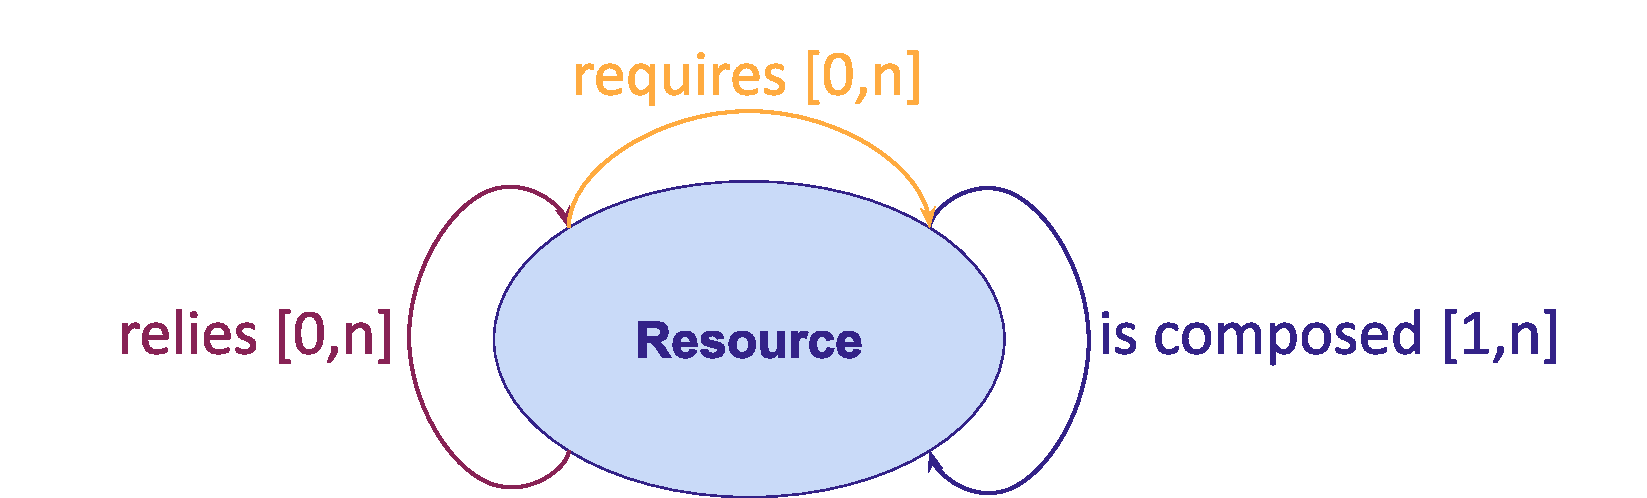
\includegraphics[width=0.7\textwidth]{figs/pdf/classification.pdf}
    \caption{The different dependencies}
    \label{fig:dependencies}
  \end{figure}



\subsubsection{Requirement}

Requirement defines a relationship between two resources that is not
critical for the survival of either of the resource but rather is a
necessary link during a particular operation.
%
The operation can be any operation performed upon either of the
resource.
%
While performing the operation the link is vital and if the link is
severed the resultant operation will terminate and it will not
succeed.
%
If the link is maintained and no external factors affect the
operation, the operation will be a success and after this the link
between these resources is insignificant.
%
Hence, a broken link after the operation does not affect either of the
resource. An example for \os is a VM requires an image, for the
creation operation.

\vspace{-15pt}
\subsubsection{Reliance}

Reliance defines a relationship between two resources that is critical
for the survival of either one of the resource or both.
%
If the link between these resources is cut at some point during the
lifetime of these resources it will impact the existence of the
resources and can lead to a failure condition.
%
Involved resources are independent and one resource cannot alter the
other resource.
%
For example, in \ks, a pod, when created with a secret, relies on this
secret.

\vspace{-15pt}
\subsubsection{Composition}
Composition consists of intrinsic dependencies between resources: the
life cycle of the two resources are linked.
%
The creation of resource A implies the creation (and respectively the
destruction) of resource B.
%
Composition is obviously wider than just two resources as one resource
can be linked to a collection of other resources, which in their turn
can also depend on sub-resources.
%
For example, in \os a stack can be composed of VMs, and in \ks, a
deployment is composed of pods.


\subsection{Creation patterns for replication operations}

\begin{figure*}[htbp]
  \centering
  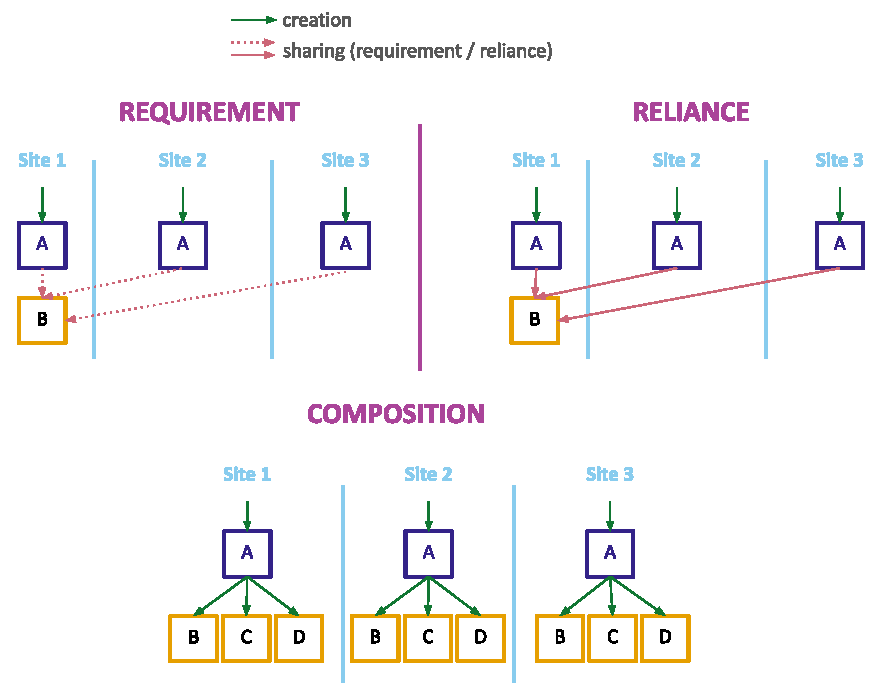
\includegraphics[width=0.76\linewidth]{figs/pdf/behaviors.pdf}
  \caption{Behaviors to observe following the dependencies}
  \label{fig:patterns}
\end{figure*}

As mentioned, the goal of the relationship model is to ensure that
Cheops operations are done thoroughly when the manipulated resource is
not elementary, but depends on other resources.
%
We discuss in this paragraph the various cases.

\begin{description}
\item[Requirement]%Under this relationship, in order to create a resource A, another resource is \emph{required}: resource B.
  For a replication scenario, the user have the choice to first
  replicate B everywhere A will be; in this case, the creation of A
  can be executed without specifying the location of B, it will be
  executed locally on each site.
  %
  The other choice is to specify the dependency in the creation
  request, which is represented in \autoref{fig:patterns}.
\begin{enumerate}
\item Using the sharing operator in the scope, the user specifies that
  a resource B required is on $Site 1$.
\item Cheops intercepts the request to get a resource from another
  site when it will be sent by the service needing it.
\item Cheops transfers the request to get resource B from $Site 1$.
\item Resource B is received and the usual flow is executed.
\item Since Resource B is only required for some operations, this
  dependency is stored in Cheops database for further usage (in these
  operations).
\end{enumerate}


\item[Reliance] This relationship follows a similar approach from
  requirement for replication.
  %
  The difference is with the involvement of Resource B through the
  life span of Resource A.
  %
  At any point if Resource B fails for both collaborations, resource A
  will result in a failure state.
  %
  The primary objective being to preserve the strong relationship
  between Resources A and B, Cheops needs to ensure the
  reachability of Resource B.

  As before, a user can still replicate Resource B to ensure that
  Resource A will not suffer from a network partition.
  %
  Otherwise, the process is the same as the requirement, except for:
  first, the dependency information needs to be stored in Cheops
  database for resource B to warn users against resources failures in
  replicas in case of a deletion of B.
  %
  Second, Cheops needs to warn the users of affected resources
  (replicas of resource A) in case of network partition that affects
  B, because they will be in a failure state.

\item[Composition] For replication scenario, a copy of resource A is
  created on the involved sites which in turn creates resources B, C
  and D on each of these sites with a \emph{cascading effect} from the
  normal, local execution of the creation of A.
  %
  An update on resource A for a secondary layer resource B, C or D is
  propagated across the involved sites and also follows normal
  execution on each site.
  %
  Network split brain is managed through the Raft protocol that
  ensures eventual consistency between all replicas.

\end{description}

Though this classification is still mainly theoritical, with some
implementations being currently studied, the implementation of the
rest of the approach will be presented in the next chapter.


\chapter{Cheops, our solution to push Cloud Applications to the Edge}
\label{chap:cheops}

In this chapter, I will present the implementation of the global
approach, and what we achieved to have our service mesh dedicated with
the purpose of pushing applications to the Edge by managing their
geo-distribution.
%
This service mesh is called Cheops.


\section{Towards a full implementation of our approach in Cheops}
\label{sec:cheops-v1}

In the appendix (\autoref{chap:first-approach}), I present the first
version of the implementation, that was a first step towards our
current approach.
%
In this section, we will discuss the current implementation, which is
still under development.

Cheops is a service mesh, with a proxy intercepting the request for
each service as the data plane.
%
The control plane is deployed on each site, as a service, as it is one
more service of the application instance.
%
In the rest of the manuscript, I will refer to ``Cheops'' as the
Cheops service deployed on each site; they all communicate between
each other to allow for collaboration, forming a service mesh with the
proxies.
%
Each of them maintains a catalog of the service instances on its site
to know how to contact them locally.
%
Each Cheops knows its neighbours and contact only the other Cheops
involved in a request, and they are responsible to contact the
involved services with their local catalog.
%
More importantly, to keep it generic, Cheops considers each type of
resources as black boxes.


In the next figures, we do not present the specific involved
endpoints, as the important part is the services involved.
%
Each service is shown as a rectangle, named as $Service X_i$ with
$Service X$ the name of the service and $i$ the identifier on the site
where it is located.
%
The proxies are represented as an oval around the services.
%
The Cheops databases are represented only when they are necessary.
%
Manipulated, involved resources are pictured as a small circle on
each service.

\subsection{Implementation of collaborations}
\label{subsec:collab-implem}


We will first detail how the three collaborations were implemented in
\emph{Cheops}, or at least some overview on how they should be
implemented.
%

\subsubsection{Sharing}

Sharing was a joint work envisioned by Ronan-Alexandre Cherrueau,
Adrien Lebre, Matthieu Simonin and Javier Rojas Balderrama with a
\acrshort{PoC} named OpenStackoïd~\cite{oid, CLRB19, CDLR+20}.
%
% Thus, sharing is not implemented in Cheops for now.

As explained in the previous chapter, \emph{sharing} is the
collaboration which allows a service instance to use a resource from a
service which is not the one assigned to its application instance.
%
This is the first way of leveraging the entire infrastructure, by
distributing different resources on different sites and allowing their
use from one site on another, enforcing the collaborative-then
principle.
%
It actually also enforces the local-first principle, because it allows
the execution locally, using only resources from other sites when
required.

\begin{figure}
  \centering
  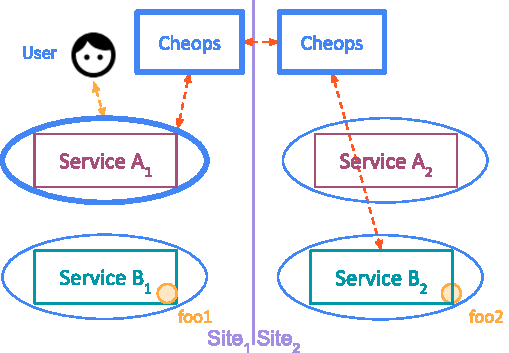
\includegraphics[width=0.7\textwidth]{figs/pdf/cheops-sharing}
  \caption{Sharing uses services instances from different sites}
  \label{fig:cheops-sharing}
\end{figure}

The typical example is getting a resource from a Service B on another
site for a Service A, the workflow presented as red arrows in
\autoref{fig:cheops-sharing}.
%
For example, if $Service A$ requires a $foo$ resource from
$Service B$, the command line given by users to request the use of
resource $foo2$ from $Service B_2$ on $Service A_1$ is:

\noindent {\small \texttt{application create a -{}-name bar -{}-sub-resource foo2 -{}-scope \{A: $Site_1$, B: $Site_2$\}}}
%

\begin{enumerate}
\item A user requests to create a resource $a$ on $Service A$ from $Site_1$
  (Service $A_1$), using a sub-resource $foo_2$ from $Service B$ on
  $Site_2$ (Service $B_2$).
\item The request is intercepted and transferred to Cheops (control
  plane).
\item Cheops extracts the scope from the request and interprets it, in
  this case, learning that it should be directed to the local
  $Service A$.
\item Cheops transfers the request to $Service A$, that executes it
  until it needs the sub-resource from $Service B$.
\item The outgoing request is intercepted, and at this point, is
  transferred to $Site_2$ for forwarding on $Service B_2$.
\item Cheops on $Site_2$ uses its catalog to find Service B endpoint
  locally and transfers the request to get $foo2$.
\item The service response (containing the resource itself) is finally
  transferred back to Service A through Cheops.
\end{enumerate}

Similarly to a local failure, if $Service B_2$ is not reachable, the
request cannot be performed.

We can see here that contrary to the intra-services collaboration we
talked about in~\autoref{sec:why-no} that requires dedicated code, our
approach use directly the response from another service instance,
which is offered by default.


\subsubsection{Replication}
\label{sssec:cheops-rep}

We will give here a first overview on how replication can be
implemented, a detailed version will be given later on, as it was the
specific collaboration I studied in our approach, and here, we give an
overview for all collaborations.
%
\emph{Replication} is the ability for users to create
and have available resources on different Edge sites to deal with
latency and split networks.
%
Replication main action is duplication: transfer the
request to every involved site and let the application execute the
request locally.
%

The operation does not simply consists though in forwarding the
request to the different instances.
%
Cheops keeps track of the different replicas in order to ensure that
future CRUD operations achieved on any replica will be applied on all
copies, maintaining eventually the consistency over time from the CRUD
point of view.
%
To do that, Cheops relies on a data scheme, called the replicant, that
links a meta-ID to the different replica IDs and their locations
(called the mapping in the previous chapter).
%
Replicants are located on every Cheops database on the sites involved
in the request to replicate, just as the replicas are located in every
application database on these same sites.


\begin{figure}
  \centering
  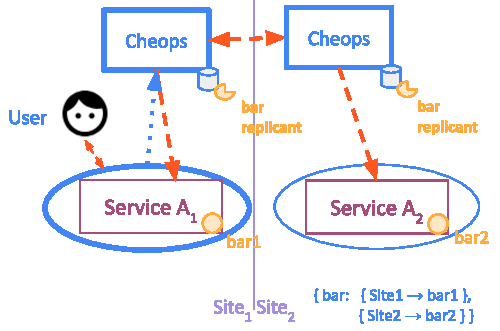
\includegraphics[width=0.8\textwidth]{figs/pdf/cheops-replication}
  \caption{Replication executes an operation on multiple instances}
  \label{fig:cheops-replication}
\end{figure}

\autoref{fig:cheops-replication} sums up the workflow to create a
replicated resource on two sites:

\noindent{\small\texttt{application create a -{}-name bar -{}-scope \{Service A:
    $Site_1$ \& $Site_2$\}}.}
\begin{enumerate}
\item A user sends a request on $Site_1$ to create two replicas of the
  \emph{bar} resource on $Service A$ from $Site_1$ and $Site_2$, \ie
  $Service A_1$ and $Service A_2$.
\item The request is intercepted and transferred to the local Cheops
  (control plane).
\item Cheops extracts the scope and interprets it, in this case, it
  needs to contact $Service A_1$ and $Cheops$ from $Site_2$.
\item Cheops creates the replicant, and passes the request to create
  it to Cheops on the other involved site ($Site_2$).
\item Both Cheops execute the request of creation of \emph{bar}
  locally, which is simply the request without the scope; the response
  is intercepted to fill the local IDs on the replicants and the
  response is transferred to the user, replacing the local ID by the
  meta-ID of the replicant.
\end{enumerate}

To provide eventual consistency, Cheops follows the Raft protocol,
with one replicant acting as the leader.
%
As for the other collaborations, it is crucial to understand that
since we manipulate the resources through the API their services
expose, we can only intervene from this point of view.
%



\subsubsection{Cross}

% This collaboration is the work from Geo Johns Antony and is still in
% progress.
% %
% It also has been preliminary and shortly studied by Karim Manaouil.
% %
% This work is given for a complete view of the approach, though the
% logic is not entirely defined, and thus subject to changes.

As mentioned earlier, Cross is not entirely mature, but has been
implemented in part in Cheops, and thus it is worth developing a bit
more.

\begin{figure}[hbtp]
  \centering
  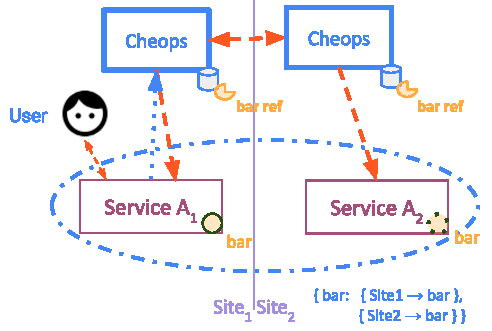
\includegraphics[width=0.8\textwidth]{figs/pdf/cheops-cross}
  \caption{Cross gives the illusion that multiple resources behave as
    a single one.}
  \label{fig:cheops-cross}
\end{figure}

%
An illustration of Cross is depicted in \autoref{fig:cheops-cross},
following this request:

\noindent{\small \texttt{application create a --name bar --scope \{Service A: $Site_1$ \% $Site_2$\}}.}

\begin{enumerate}
\item A user sends a request to create a resource specifying the
  involved sites in the Cross operation.
\item The request is intercepted and transferred to Cheops.
\item Cheops extracts the scope and interprets it.
\item Cheops creates the resource on the first site ($Site_1$) and
  passes the request to Cheops of other involved sites (here, $Site_2$
  only).
\item Cheops on $Site_2$ identifies the extended resource and creates
  an identifier within Cheops to forward to the deployed resource site.
\end{enumerate}




\subsection{Cheops architecture}
\label{ssec:cheops-archi}

% \todoref{cf  https://mqtt.org/}


The global architecture of our proof-of-concept is depicted in
~\autoref{fig:Cheops-architecture}.
%
Cheops follows a modular approach, composed of various microservices,
which are linked together through REST API protocol.
%
There is one Cheops per site and they monitor known Cheops
through heartbeats.

For redirection purposes, each Cheops has its own internal registry.
%
First, it stores information about its own site: the addresses of each
application service endpoint as a catalog or registry.
%
Second, it keeps the addresses of its Cheops neighbours to know where
to transfer the requests when needed.
%
%
Cheops never intercepts requests coming from a Cheops to an
application service to avoid looping.


\begin{figure}[hbtp]
  \centering
  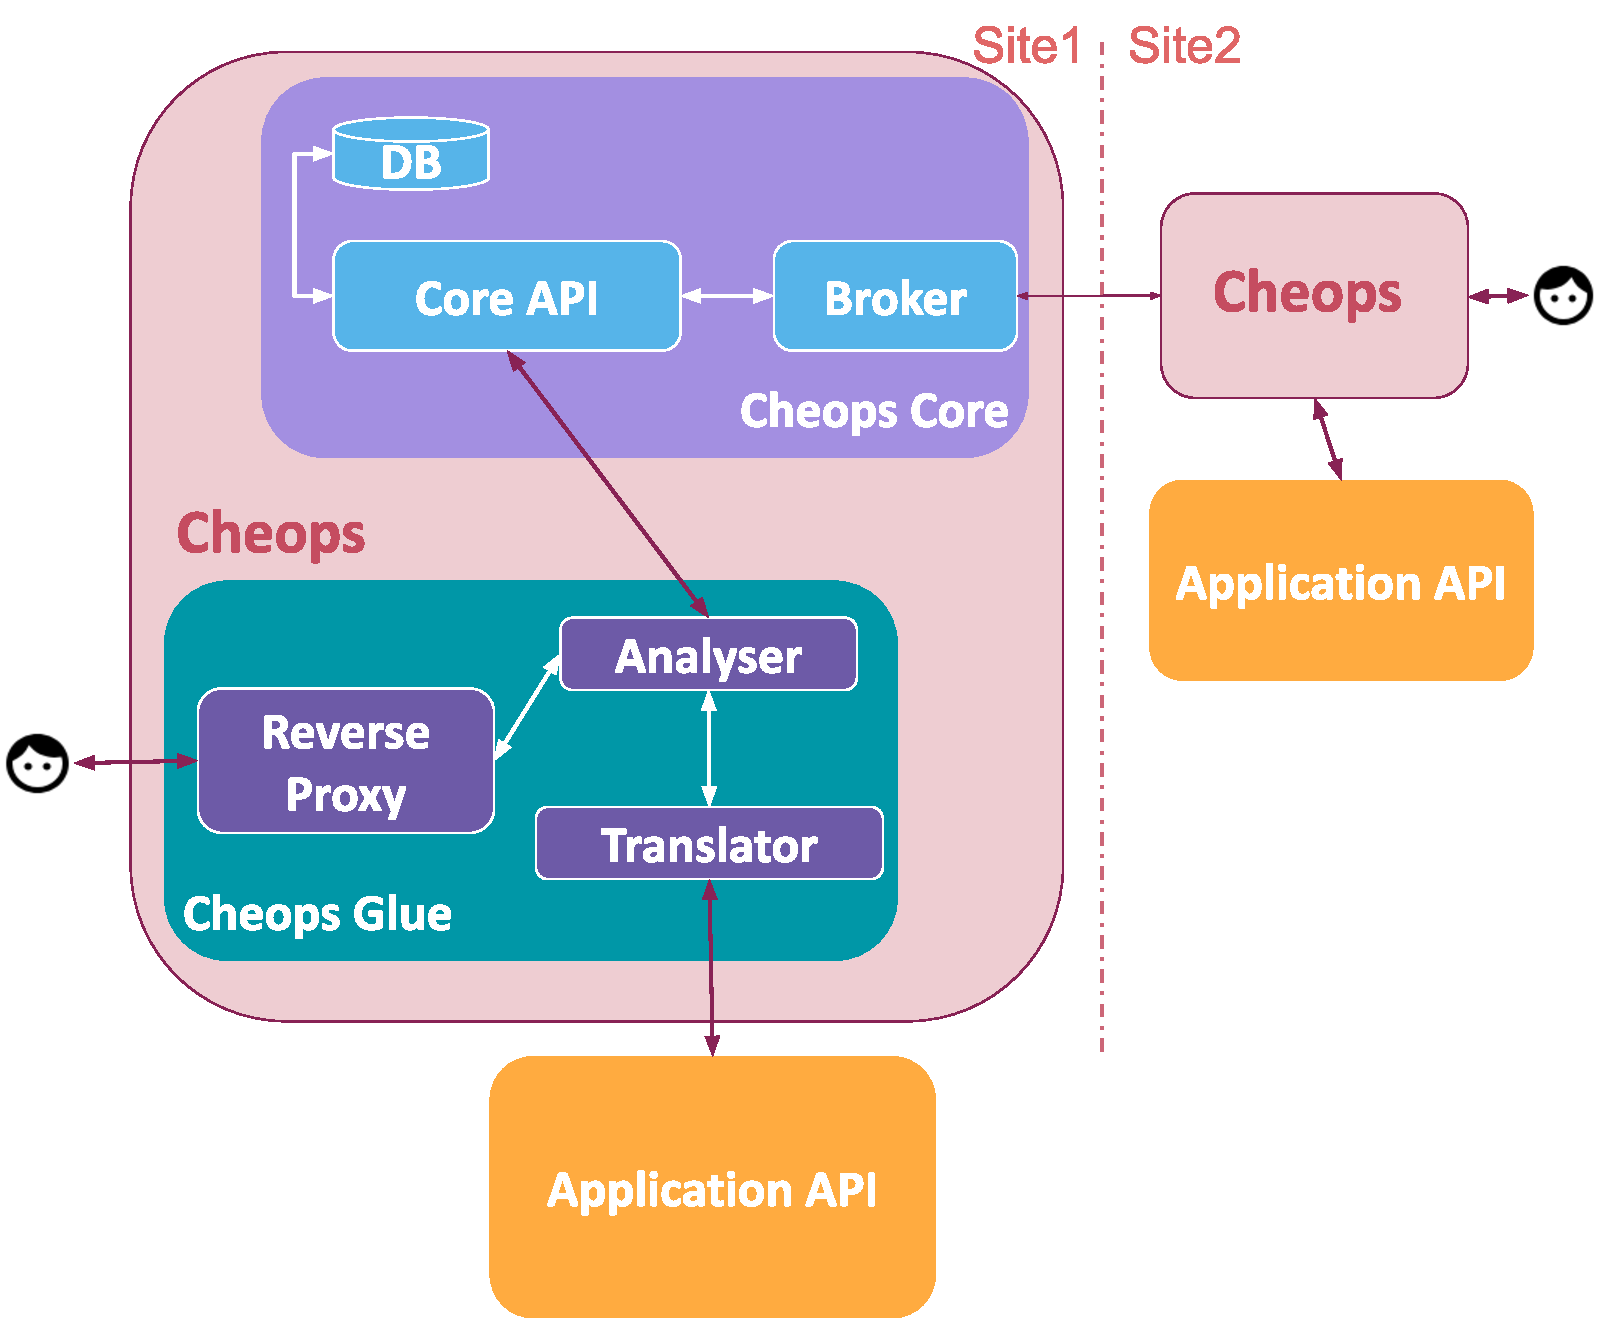
\includegraphics[width=.75\linewidth]{figs/pdf/cheops-architecture}
  \caption{Cheops architecture}
  \label{fig:Cheops-architecture}
\end{figure}
%

\subsubsection{Cheops internals}
%
The Cheops control plane is divided into two main components which are
Cheops Core API and Cheops Glue.
% The modular approach promises integration of various frameworks

\begin{description}
\item{\textbf{Cheops Core}} is the primary building block of Cheops.
  %
  It encapsulates the communication module, interface module (Core
  API) and the database.
  %
  The communication module provides the link between multiple Cheops
  instances, thus creating and maintaining a service mesh around the
  various involved clusters.
  %
  Since Cheops focuses on minimizing intrusive code changes of a
  deployed application, this module plays a significant role, while
  addressing the collaboration features of Cheops.
  %
  This module also communicates with the the Core API module in the
  Core.
  %
  The Core API is a management module created to interconnect all the
  services inside Cheops.

\item{\textbf{Cheops Glue}} is the second module of Cheops.
  %
  This module is designed to help Cheops Core translate Cheops API
  requests into the respective application API and vice-versa.
  %
  Core is designed to handle agnostic API requests which are
  irrespective to all the applications.
  %
  Cheops needs to convert these requests into application
  understandable API patterns.
  %
  Since each application has its own pattern for intercepting API,
  Glue is developed with respect to individual applications such as
  Openstack, Kubernetes, etc.
  %
  Thus, this module is not generic to every approach and has to be
  implemented to translate the requests, but still allows the
  externalization of geo-distribution concerns.
  %
  Glue acts as a first layer communication between users and Cheops by
  intercepting the data from the default CLI from the respective
  application using \scl.
  %
  The analyzer service in Glue evaluates the request and converts it
  into a generic request understandable by the Cheops Core API
  service.
  %
  On the other side, Cheops Glue provides a translator service which
  converts the requests received from the Cheops Core API service.
  %
  Cheops Glue will also manage the creation of extra business logic for
  divisibility property of cross collaboration
  (see~\autoref{fig:cheops-cross}) for specific types of resource.
  %
  The Glue also handles the network requirements and implements the
  relationship model (that we will only discuss in the future work
  part of the conclusion).
%Implementing a relationship model for resources dependent on the type of resource which requires a dedicated logic which will handle this.
\end{description}

The design of Cheops architecture is focused on a modular design
which makes it easier to manage and distribute.
%
It also provides the flexibility of enhancing each component or
individual service to scale it during peak usages.
%
It is available for any request specifying the usage of its hosting
site when it is not disconnected from the network (not offline) and
the users are also able to control this instance locally, making it
available at any time.
%
Cheops obviously offers the three collaborations proposed earlier.
%
It manages each collaboration without the need to modify anything in
the deployed application.
%
Finally, it maintains the consistency of the deployed applications
across the locations.




% \section{Scope-Lang interactions with Cheops}
% \label{sec:cheops-scl}



\section{A deeper dive into the replication}
\label{sec:cheops-replication}



As previously introduced, replication is the ability to create and
maintain identical resources on different sites: an operation on one
replica should be propagated to the others, dealing with faults and
disconnections and maintaining CRUD consistency based on our eventual
model.
%
Other consistency policies~\cite{ATB+16, ZW15} could be envisioned,
but let as future work as they do not change the general concept of
\scl/Cheops.
%
To get a better understanding of the point of replication, imagine a
user who needs a huge resource (like an ISO image) both at home and at
work.
%
The resource can be replicated at creation on both sites and it will
be the only time when the entire resource will go through the network.
%
This saves a lot of bandwidth, and is especially useful if there is a
partition between both sites, or if the user wants to work offline.


\subsection{Replication model}

A lot of this model has been discussed in~\autoref{ssec:scl-rep}
and~\autoref{sssec:cheops-rep}, so we will avoid as much as possible
repetitions, unless it can be explained differently for a better
understanding.

A replicant is basically a meta-identifier we generate along with a
list of mappings $site \rightarrow local\_identifier$ and a service
name (or identifier).
%
A replicant can thus be implemented for example as:

$ { meta\_identifier: [ site_n: local\_identifier_n, ...], service\_name} $

% We only store the location (site) of the replica and not the service
% used since it is possible to deduce the service with the incoming
% request.
% %
% This is subject to change depending of the evaluation of our
% prototype. We could store also the involved service and/or the type of
% resource involved.

It is important to know that for now, the service name has not been
used in the current implementation as the request given has been
enough to transfer to the correct service.

These replicants are stored in a database co-located to the Cheops
agents.
%
A copy of the replicant is stored on each site where its replicas are
located (the sites involved in the replication).
%
Cheops has an API of its own to allow the user to check the state of
operations, sites and inspect replicants.


\subsection{CRUD execution workflow}


First, to define what is the creation, update or delete workflow, we
have to define what they do in our consistency model and what are
their boundaries.

In replication, resources are only considered as black boxes seen only
as the API allows it, and thus the consistency maintained only by the
operations allowed by the API (usually CRUD operations).
%
Any modification made internally on one site by the application
without using the API cannot be expected to be replicated to the other
replicas.
%
Furthermore, any modification made on those replicas through the API
will be applied eventually to the other replicas.

%
The creation of resources replicated in an eventual consistency
implies that all replicas are identical at creation and will be
created eventually.
%
The update of resources created with the replication in an eventual
consistency implies that all replicas will be updated eventually,
whether the user specifies a scope or not in its request.
%
It is the same as updates for deletes.

About the boundaries, the operation obviously begins when the user makes
the request.
%
But for the end, we could consider that an operation ends either when
there is one response and is returned to the user, or when the
operation is executed on every site.
%
In an eventual consistency model, the latter (the operation done on
every site) can come a lot later than the first response.
%
%This is why we chose to decide for

%
It is important to know what happens in case of failure (partition,
disconnection, server failure) during the execution until the first
response, but also after, because the operation must be executed on
our replicas at some point.


In terms of the user view, the first response to arrive goes to the
user before it might be applied everywhere, so it is the
responsibility of the user to check with a request to Cheops or
directly to involved services and sites to know where the creation or
updates are already applied.
%
Users cannot assume because they received the answer the operation as
already been applied everywhere, some sites may have difficulty to
execute the request or may be even down.


\subsubsection{Creation}

The replication process to create a resource on $App_1$ and $App_2$
has already been detailed in~\autoref{ssec:scl-rep}
and~\autoref{sssec:cheops-rep}.
%
Therefore, we will not develop it further in this part, and the reader
can refer to these parts to know about it.




\subsubsection{Read}

%
Since the replicas are the same from the API level view, on a
probability of a replica not updated yet, read one replica or another
should not be different, so only one is needed to be returned.
%
Therefore, the process of reads is straightforward; to access a
specific resource, users must either request their site where one of
its replicas is (local-first) or specify in the scope on which
location a replica of the resource to read is (collaborative when
needed).




\subsubsection{Update}

After the creation of replicas, every request made to update (or
delete) is filtered to check if the id given corresponds either to a
replicant meta identifier or a local replica identifier.
%
Once again, this process is really long, so it is pretty costly, but
it ensures the consistency of the approach.
%
Ideally, it should be configurable, so the users can take
responsibility for the divergence of state in the replicas if they use
local replicas identifiers and everything is not analyzed.
% If it is, the request is transfered to every sites
% containing one of the replicas before being executed.
%
The process is quite similar to the creation, but does not generate a
new replicant or change an existing one.
%
It only applies an update to replicas and update the logs of
replicants.
\begin{enumerate}
\item
  A request for an update of a previously created replica is
  addressed to the endpoint of a service of one application instance.
%% \item
%%   Cheops uses its list of drivers to check which one to use, and sends
%%   the request to the correct one.
\item Cheops checks if the ID in the request exists in the replicant
  database.
  %
  If not, the request is sent back to the service to be executed.
  %
  If it is, the request is transferred to the Cheops agent storing
  the replicant leader.
  %
  It gets the corresponding replicant to find all replicas (and thus
  sites) involved.
  %
  The leader sends a vote to the replicants to have a consensus on the
  request.
  %
  When it gets the consensus, the operation is stored in its log.
\item The request is copied as many times as necessary (with the
  corresponding local identifier from the mapping so it will work
  properly on the different involved sites) and sent to the Cheops
  agent of involved sites.
\item
  Local Cheops agents send the request to the corresponding service on
  their site, which executes the request normally.
\item
  Each Cheops agent sends back the response to the Cheops agent where
  the replicant leader is.
\item This agent sends back the first response to the user, once
  again, with the meta-identifier where the local-identifier would be
  expected to notify the user that the replicas were updated.
\end{enumerate}



\subsubsection{Delete}

As for the update, a delete on replicas can be identified either by a
local identifier or the meta identifier.
%
The process is identical as the update's.

It is important in this subsection that adding replicas to a set of
pre-existing replicas situations have not been fully studied for
implementation yet, though they have been considered.
%
Conversely, the removal of a replicant from the set is important in
the processes of dealing with faults.


\subsection{Dealing with faults}


We define a fault as: a partition of network on an involved site
(disconnection), or a failure from this site, whether it is shut down,
out of order, or if the request cannot be executed for any reason (not
enough memory to create a resource for example).

It is also important to mention that if the site where the user sent
its request is faulty (does not work in any of the aforementioned
way), the request obviously cannot be executed.
%
The user can make the request to a more distant site, but this is one
of the advantage of replication.

Moreover, the ``during an operation'' can refer to two distinct
phases.
%
As we discussed before, the end of an operation can be seen
as: when a replica has been created/updated/deleted and the user has
been notified, and when the operation is applied to all replicas.
%
So ``during an operation'' is between the request of the user and
before one of these ends.
%
In our consistency model, this conveys no difference to the process.
%, but it does have an impact on the availability and state

If a site fails where a replica is supposed to be, other Cheops will
be informed due to its heartbeat (or rather lack of).
%
Any other operation received by the leader will then be retried
according to the log when the site comes back again.
%
Therefore, a site is considered to be eventually available again
unless it is removed.
%
If a site is removed from the system, every site that was hosting a
replica must delete the site from its mappings (from the replicant).
%
The leader will be in charge of this particular task, sending a
request to update the replicant.


\begin{description}

\item [Faults during operations]


The operation will be applied \emph{eventually} on all involved
sites.
%
This eventual consistency uses a consensus protocol, and in our
case, an implementation of Raft~\cite{OO14}.
%
For example, the leader's log allows to replay operations that are not
yet applied.
%
It is the responsibility of Cheops hosting the leader to ensure that
operations are applied eventually, by checking regularly operations
that have not been yet applied.


\item[Faults while there are replicas but not particular operation]

When a site fails while there are replicas somewhere without any
particular operation running, no heartbeat is received by other Cheops
agent and the replica is considered unavailable temporarily.

If a site where a replica is was partitioned at some point but could
be used locally, only read queries can be made, and these reads might
be stale (not be up-to-date to the operations that have been made on
other replicas). When rejoining the cluster, operations will be
applied on the site so it is up-to-date thanks to the leader's log.

\end{description}



\section{Testing Cheops replication}
\label{sec:validation}

We demonstrated the feasibility of our proposal on the Kubernetes
ecosystem.
%
The feasibility for the collaborations were studied for replication,
in which we manipulated replicated pods across two sites.
%
% Some experiments were made on the cross collaboration, too, but, since
% it is not the focus of this manuscript, we will not detail those here.


The experiments have been performed over two sites of the Grid'5000
experimental testbed~\cite{grid5000}, as it was used for the first
version of Cheops (see in the
appendix,~\autoref{chap:first-approach}).
%
The sites were completely independent of each other and located on two
sites of the infrastructure, namely Nantes and Rennes.
%
On each site, we deployed a Kubernetes cluster, each composed of one
master and one worker node, as well as Cheops.


%

\subsection{Current technology stack}


Cheops was deployed onto each site alongside an instance of the
application (Kubernetes), creating a \acrshort{P2P} service mesh
structure between these applications.
%
The primary goal was to create an initial development efforts as per
the architecture ~\autoref{fig:Cheops-architecture}.
%
These efforts provided the functionalities we proposed to create a P2P
service mesh, integrate collaboration mechanisms and flexibility to
extend to multiple applications.


For the initial study, Cheops was built on Golang, since it is very
adaptable to server-side scripting.
%
In order to create the service mesh, Cheops relies on a message broker
which provided P2P capabilities and a reliable messaging protocol.
%
Advanced messaging queuing protocol (AMQP) was chosen for our design of
the Cheops-to-Cheops communication (communication module of the Core).
%
RabbitMQ\footnote{\url{https://www.rabbitmq.com/} - Accessed
  2022-10-09} with P2P and AMQP messaging pattern were used for this
purpose.
%

For the database, the main requirement was to find a free and open
source database (for easier adoption) which could replicate the data
based on individual attributes.
%
After a survey, the conclusion made was that no particular database
existed which met all the required characteristics, and thus
ArangoDB\footnote{\url{https://www.arangodb.com/community-server/} -
  Accessed 2022-10-09} was chosen to be integrated into Cheops, to
allow us to have a NoSQL document store that could keep different
types of data.
%


The next component needed was the one that can intercept the users
requests in order to identify the request patterns and especially to
be able to get the scope in requests.
%
HAProxy\footnote{\url{https://www.haproxy.com/} - Accessed 2022-10-09}
was chosen to provide a lot of flexibility in order to integrate
between the application and Cheops.
%
\emph{Nonetheless, it is crucial to know that though we deploy HAProxy
in the current \acrshort{PoC}, we do not intercept requests and we
only use Cheops API to make the request.}
% \todomore{https://www.haproxy.com/blog/layer-4-and-layer-7-proxy-mode/}
% \todomore{we only use one proxy in lieu of one for each service}


In more details for the replication,~\autoref{fig:replicant} presents
the model for the Replicant structure, which is composed partly of a
slice (re-sizable array) of Replica objects.
%
In the Replica struct, there are information on the Site (name in our
case, but it could be an ID of a site for very large scale) on which
the Replica is, the ID of the local resource, and a Status that is not
used for now, but was added as a maybe simpler way to know if one
replica is reachable or not.
%
In the Replicant struct, we store the Meta-ID as expected, the
different Replicas (from the above struct), a Boolean to know if this
particular Replicant is the leader of the Replicants, and finally the
Logs of the different operations executed on the Replicas to maintain
consistency.
%
For those who are not used to Golang, the json information at the end
of the fields of the structures is for encoding and decoding to and
from JSON, so they can be passed with a REST request.




\begin{figure}
  \centering
  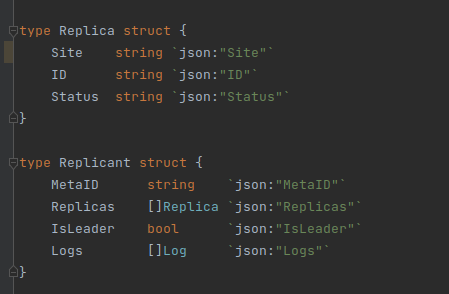
\includegraphics[width=0.8\textwidth]{figs/png/replicant-model}
  \caption{Actual replicant model in Cheops code.}
  \label{fig:replicant}
\end{figure}




\subsection{Experiments}
%We performed the feasibility study for the collaborations~\autoref{sec:collabs}. Replication and Cross were tested out on the Kubernetes framework in Grid'5000 testbed.

The artifact we used for the experiments is available on the Cheops
project page\footnote{\url{https://gitlab.inria.fr/discovery/cheops/}}
(around 3k lines of code).
%
It is a joint work from Geo Johns Antony and myself.


The goal of the experiments we performed was mainly to validate the
expected behavior and genericity on simple requests.
%
Further experiments are still needed, and as mentioned, some
experiments on cross have also been performed but will not be
presented here.


\autoref{table:replication} presents the commands tested and their
results.
%


\begin{table}[htbp]
  \centering
  \setlength{\tabcolsep}{10pt} % Default value: 6pt
  \renewcommand{\arraystretch}{1.3}
  \begin{tabular}{|l|c|l|}
    \cline{1-3}
    \multicolumn{1}{|c|}{Operation}                                                                        & \multicolumn{1}{c|}{Location} & \multicolumn{1}{c|}{Result} \\ \cline{1-3}
    \begin{tabular}[c]{@{}l@{}}\verb|kubectl create pod purple| \\ \verb|    --scope{Site1&Site2}|\end{tabular} & Site1   & Pod \emph{purple} created on Site1 and Site2  \\
    \cline{1-3}
    \begin{tabular}[c]{@{}l@{}}\verb|kubectl create pod violet| \\ \verb|    --scope{Site1&Site2}|\end{tabular} & Site2   & Pod \emph{violet} created on Site1 and Site2  \\
    \cline{1-3}
    \verb|kubectl get pod violet| & Site1  & Pod \emph{violet} from Site1 is displayed \\
    \cline{1-3}
    \verb|kubectl get pod violet| & Site2   & Pod \emph{violet} from Site2 is displayed  \\
    \cline{1-3}
  \end{tabular}
  \caption{Experimentations on Kubernetes - replication.}
  \label{table:replication}
  % \vspace{-15pt}
\end{table}

We created one pod \emph{purple} and one pod \emph{violet}
respectively on \verb|Site1| and \verb|Site2|, with the scope
specifying to create those pods as replicas on both sites.
%
This means we should have a \emph{purple} on \verb|Site1| and
\verb|Site2|, and the same for the pod \emph{violet}.
%
This corresponds to the commands
\verb|kubectl create pod purple --scope{Site1&Site2}| and
\verb|kubectl create pod violet --scope{Site1&Site2}|, respectively on
\verb|Site1| and \verb|Site2|.

Then we requested the pods \emph{violet} from each site to check if
they were present.
%
This corresponds to the commands \verb|kubectl get pod violet| on both
\verb|Site1| and \verb|Site2|.

%
Though this set of requests tests really basic functionalities, we
were able to ensure that the \emph{create} and \emph{get} operations
were working as intended.
%

Additional experiments are under progress to test \emph{update} and
\emph{delete}, as well as scenarios on the behavior of replicas in
case of network split to check the consistency.
%
A study on different types of resources to better check the genericity
is also required.
%
Especially, we used Kubernetes for this, because the approach has
already been tested on \os, but we did not try this particular
\acrshort{PoC}, so this could be a further important test.


\chapter*{Summary of the approach}
\label{chap:summary-cheops}


To fulfill the requirements stated in~\autoref{sec:principles}, using
different existing technologies and means, Cheops and \scl are a
solution to bring existing, service-based Cloud applications to the
Edge.
%
The main goal is allow any of these applications to be run on Edge
infrastructures without changed in their code, by taking into account
the properties of the Edge.


Cheops a service-mesh which main functionality is to manage the
geo-distribution of the Edge sites and the resources of the
applications.
%
Scope-lang allows users to define the execution location and
collaboration in their requests \textbf{dynamically},
\textbf{on-demand}.

With the application deployed on each site, the solution answer the
\textbf{local-first} requirement automatically.
%
The different collaborations, of which we presented three, namely
sharing, replication and cross, fulfill the
\textbf{collaborative-then} requirement.

By externalizing the geo-distribution concerns, the approach is
\textbf{non-intrusive}, and it is as \textbf{generic} as possible
by only considering resources as black boxes and using the application
API, with only the Cheops glue specific to the applications.

The Cheops service mesh functions in a \textbf{decentralized} and
\textbf{P2P} manner, and is designed with autonomous sites and some
collaborations, to be \textbf{resilient to network partitions}.
